\chapter{Ejemplos NodeJs}

Esta primera parte de la práctica consta de cinco ejemplos que sirven para aprender
el funcionamiento de NodeJs y Mongo.

Lo primero que hay que hacer es instalar las dependencias con \texttt{npm} o con \texttt{yarn},
el que escojamos para esto será el que usemos para el resto de la práctica.

Para simplificar la ejecución de los ejercicios se añadido órdenes de ejecución a
\texttt{package.json}.

\section{Ejemplo 1: Hola mundo!}
Lo primero es iniciar el servidor desde la terminal con:
\begin{lstlisting}[language=sh]
	yarn helloworld
\end{lstlisting}

Después abrimos en el navegador la dirección \texttt{127.0.0.1:8080} o \texttt{localhost:8080},
y se mostrará la cadena ``Hola mundo'' en la página, este mensaje se puede cambiar si modificamos
la llamada \texttt{response.write()}.

\section{Ejemplo 2: Calculadora}
Iniciamos el servidor ejecutando en la terminal:
\begin{lstlisting}[language=sh]
	yarn calculadora
\end{lstlisting}

Después debemos abrir la misma dirección, esta vez debemos añadirle argumentos para
que imprima el resultado; se escribiría entonces de la siguiente
forma: \texttt{127.0.0.1:8080/operacion/numero1/numero2}.

Las operaciones que soporta son: sumar, restar, producto y división.

\begin{figure}[!ht]
	\begin{center}
		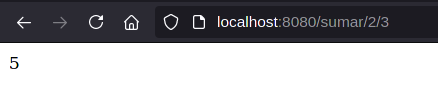
\includegraphics[scale=0.5]{calculadora.png}
	\end{center}
\end{figure}

\section{Ejemplo 3: Calculadora-web}

Iniciamos el servidor ejecutando en la terminal:
\begin{lstlisting}[language=sh]
	yarn calculadora-web
\end{lstlisting}

Este ejemplo proporciona la misma funcionalidad que el anterior, salvo que en vez de
tener que escribir las operaciones en la barra de búsqueda, se nos ofrece una interfaz
gráfica en la página.

\begin{figure}[!ht]
	\begin{center}
		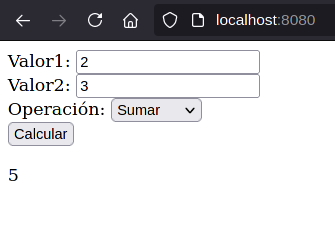
\includegraphics[scale=0.5]{calculadora-web.png}
	\end{center}
\end{figure}

\section{Ejemplo 4: Connections}
Iniciamos el servidor ejecutando en la terminal:
\begin{lstlisting}[language=sh]
	yarn connections
\end{lstlisting}

Con este ejemplo abrimos una conexión a \texttt{WebSocket} con \texttt{socket.io}

Cuando se conecte un cliente se mostrará por consola, y al desconectarse igual. El servidor
envía ``Hola Cliente'' cuando uno se conecta y si sigue abierta la ventana y se apaga el servidor
se mostrará el mensaje ``¡El servicio ha dejado de funcionar''

\begin{figure}[!ht]
	\begin{center}
		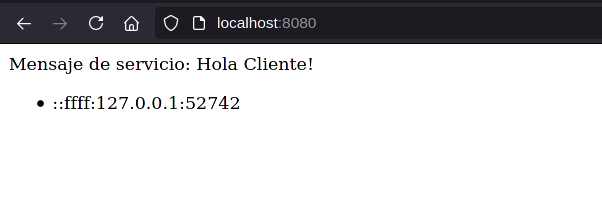
\includegraphics[scale=0.5]{hola.png}
	\end{center}
\end{figure}

\begin{figure}[!ht]
	\begin{center}
		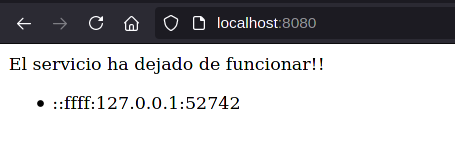
\includegraphics[scale=0.5]{desconexion.png}
	\end{center}
\end{figure}

\section{Ejemplo 5: Mongo Test}
Iniciamos el servidor ejecutando en la terminal:
\begin{lstlisting}[language=sh]
	yarn mongo
\end{lstlisting}

En este ejemplo hacemos la primera aproximación para conectarse a una base de datos de MongoDB,ex.de
es necesario tener instalado y activado el servicio.

Al ejecutar el ejemplo crea una base de datos llamada ``pruebaBaseDatos'' y
crea la colección ``test'' en ella. El cliente y el servidor se conectan por
\texttt{Socket.io} y la base de datos almacena las direcciones de los
clientes que se conectan.
